\documentclass[12pt,a4paper]{article}

% ====== ENCODING & IDIOMA ======
\usepackage[utf8]{inputenc}   % entrada UTF-8
\usepackage[T1]{fontenc}      % output con font T1 (acentos correctos)
\usepackage[spanish]{babel}   % idioma español (división silábica, títulos, etc.)


% ====== DISEÑO DE PÁGINA ======
\usepackage{geometry}
\geometry{margin=1in}
\usepackage{setspace}
\onehalfspacing
\usepackage{parskip} % mejor separación entre párrafos
\usepackage{fancyhdr}
\usepackage{titlesec}

% ====== GRÁFICOS, TABLAS, CÓDIGO ======
\usepackage{graphicx}
\usepackage{float}       % [H] para fijar figuras/tablas
\usepackage{booktabs}    % tablas bonitas
\usepackage{caption}
\usepackage{xcolor}
\usepackage{listings}    % bloques de código simples
\lstset{
  basicstyle=\ttfamily\small,
  breaklines=true,
  frame=single,
  columns=fullflexible,
  showstringspaces=false
}
\usepackage{amsmath}

% (Opcional) Si quieres hipervínculos en el PDF
\usepackage[hidelinks]{hyperref}

% ====== ENCABEZADO/PIE ======
\pagestyle{fancy}
\fancyhf{}
\fancyhead[L]{IC-6200 Inteligencia Artificial}
\fancyhead[R]{II Semestre 2025}
\fancyfoot[C]{\thepage}

% ====== FORMATO DE SECCIONES ======
\titleformat{\section}{\large\bfseries}{\thesection.}{0.5em}{}
\titleformat{\subsection}{\normalsize\bfseries}{\thesubsection.}{0.5em}{}

% ====== RUTAS DE IMÁGENES ======
% Ajusta si tus figuras están en otra carpeta:
\graphicspath{{./}{./bench/}}

% ====== DOCUMENTO ======
\begin{document}

% -------- PORTADA --------
\begin{titlepage}
    \centering
    
\includegraphics[width=0.5\textwidth]{img/logo-tec.png}
    \vspace{1cm}

    {\LARGE Instituto Tecnológico de Costa Rica \par}
    \vspace{0.5cm}
    {\Large Escuela de Ingeniería en Computación \par}
    \vspace{0.5cm}

    {\LARGE \textbf{IC-6200 – Inteligencia Artificial}}\\[2cm]

    {\huge \textbf{Tarea Corta 2 – Algoritmos Geneticos}}\\[3cm]

    \textbf{Estudiantes:}\\[0.3cm]
    Pablo Mauricio Mesén Alvarado -- 2023071259\\
    Samir Fernando Cabrera Tabash -- 2022161229\\
    Luis Gerardo Urbina Salazar -- 2023156802\\[1.5cm]

    \textbf{Profesor:}\\[0.3cm]
    Kenneth Roberto Obando Rodríguez\\[1cm]

    24 de septiembre de 2025 \\[0.3cm]
    II Semestre 2025
    \vfill
\end{titlepage}

% -------- ÍNDICE (opcional) --------
 \tableofcontents
 \newpage

\section{Resumen ejecutivo}

Este trabajo implementa un algoritmo genético (AG) para resolver el problema de control de CartPole en el entorno Gymnasium. Se evaluaron 27 configuraciones experimentales combinando tamaños de población (10, 20, 30 individuos), números de generaciones (10, 30, 50) y tres métodos de crossover.

La metodología emplea cromosomas de 4 genes (pesos) correspondientes a las variables de estado del CartPole. La función de fitness se basa en el número de pasos que el agente mantiene el equilibrio (máximo 500). Se implementó paralelización para optimizar tiempos de evaluación, selección elitista del 20%, y mutación gaussiana con tasa del 10\%.

Los resultados muestran que múltiples configuraciones alcanzaron el fitness máximo de 500 pasos. Las configuraciones con mayor número de generaciones (50) y poblaciones más grandes (30) presentaron mayor consistencia en la convergencia. Los algoritmos genéticos resultaron efectivos para este problema de control, proporcionando una alternativa viable a métodos tradicionales de aprendizaje por refuerzo.

\section{Introducción}

Los algoritmos genéticos son técnicas de optimización bioinspiradas basadas en los principios de la evolución natural. Utilizan mecanismos como selección, crossover y mutación para evolucionar poblaciones de soluciones candidatas hacia óptimos globales.

El problema de CartPole consiste en mantener equilibrado un poste articulado sobre un carro que se mueve horizontalmente. El agente debe aplicar fuerzas hacia la izquierda o derecha para evitar que el poste caiga. Este problema es un benchmark clásico en aprendizaje por refuerzo debido a su simplicidad conceptual pero desafío de control continuo.

Los algoritmos genéticos ofrecen ventajas para problemas de control: no requieren información sobre gradientes, pueden manejar espacios de búsqueda discontinuos, y son naturalmente paralelizables. En el contexto de CartPole, permiten evolucionar políticas de control representadas como combinaciones lineales de variables de estado.

La motivación de este trabajo es evaluar la efectividad de los algoritmos genéticos en un problema de control clásico, comparando diferentes configuraciones de parámetros y métodos de crossover. Los fundamentos teóricos incluyen la codificación de políticas como cromosomas, la definición de fitness basada en rendimiento temporal, y la aplicación de operadores evolutivos para la mejora iterativa de las soluciones.


\section{Descripción de la modalidad escogida (juego)}
CartPole-v1 es un entorno de control clásico disponible en la biblioteca Gymnasium (anteriormente OpenAI Gym). El problema consiste en balancear un poste articulado sobre un carro que se desplaza horizontalmente sobre una pista de longitud limitada.

\begin{figure}[H]
  \centering
  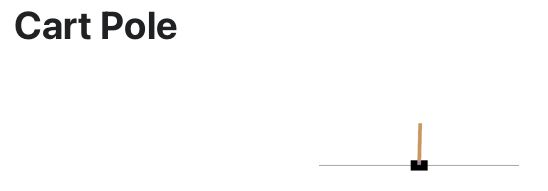
\includegraphics[width=0.6\textwidth]{img/cartPole.jpeg}
  \caption{Imagen de referencia a CartPole.}
\end{figure}

\textbf{Espacio de estados:} El estado del sistema se representa mediante un vector de 4 dimensiones:


\begin{itemize}
    \item Posición del carro: $x \in [-4.8, 4.8]$
    \item Velocidad del carro: $\dot{x} \in (-\infty, \infty)$
    \item Ángulo del poste: $\theta \in [-24^\circ, 24^\circ]$ (aproximadamente)
    \item Velocidad angular del poste: $\dot{\theta} \in (-\infty, \infty)$
\end{itemize}


\textbf{Espacio de acciones:} El agente puede aplicar una fuerza discreta:
\begin{itemize}
\item Acción 0: Empujar el carro hacia la izquierda
\item Acción 1: Empujar el carro hacia la derecha
\end{itemize}
\textbf{Función de recompensa:} El agente recibe una recompensa de +1 por cada paso temporal en que mantiene el poste equilibrado. Un episodio termina cuando:
\begin{itemize}
\item El ángulo del poste excede los ±12° de la vertical
\item El carro se sale de los límites de la pista (±2.4 unidades)
\item El episodio alcanza 500 pasos (considerado como éxito)
\end{itemize}
La dificultad del problema radica en la naturaleza inestable del sistema: el poste tiende naturalmente a caer, requiriendo acciones de control continuas para mantener el equilibrio. El desafío es aprender una política que balance efectivamente las fuerzas aplicadas al carro para estabilizar el poste mediante retroalimentación basada únicamente en el estado observable del sistema.

\section{Diseño del cromosoma y función de fitness}

\subsection{Representación del cromosoma}
Cada individuo en la población se representa como un vector de pesos 
$\mathbf{w} = [w_1, w_2, w_3, w_4]$, donde cada componente corresponde a una variable de estado del CartPole:

\begin{itemize}
    \item $w_1$: peso para la posición del carro
    \item $w_2$: peso para la velocidad del carro
    \item $w_3$: peso para el ángulo del poste
    \item $w_4$: peso para la velocidad angular del poste
\end{itemize}

Los pesos se inicializan aleatoriamente en el rango $[-1, 1]$ y se mantienen acotados en $[-2, 2]$ durante la evolución para evitar valores extremos.

\subsection{Política de control}
La política implementada es una función lineal simple:

\begin{equation}
\text{acción} =
\begin{cases}
0 & \text{si } \mathbf{w} \cdot \mathbf{s} < 0 \\
1 & \text{si } \mathbf{w} \cdot \mathbf{s} \geq 0
\end{cases}
\end{equation}

donde $\mathbf{s}$ es el vector de estado observado y $\mathbf{w} \cdot \mathbf{s}$ representa el producto punto entre los pesos y el estado.

\subsection{Función de fitness}
La función de fitness evalúa el rendimiento promedio de un individuo ejecutando múltiples episodios:

\begin{equation}
\text{fitness}(\mathbf{w}) = \frac{1}{N} \sum_{i=1}^{N} R_i(\mathbf{w})
\end{equation}

donde $N = 3$ es el número de episodios de evaluación y $R_i(\mathbf{w})$ es la recompensa total obtenida en el episodio $i$ (número de pasos hasta la terminación, máximo 500).

\section{Parámetros y configuración experimental}

\subsection{Parámetros del algoritmo genético}
\begin{itemize}
    \item \textbf{Tamaño de población:} 10, 20, 30 individuos
    \item \textbf{Número de generaciones:} 10, 30, 50
    \item \textbf{Tasa de mutación:} 0.1 (10\%)
    \item \textbf{Episodios por evaluación:} 3
    \item \textbf{Método de selección:} Elitismo (20\% de supervivientes)
\end{itemize}

\subsection{Operadores evolutivos}
\textbf{Mutación gaussiana:} Se aplica ruido gaussiano con media 0 y desviación estándar 0.2:

\begin{equation}
\mathbf{w}' = \mathbf{w} + \mathcal{N}(0, 0.2^2)
\end{equation}

\textbf{Métodos de crossover implementados:}
\begin{enumerate}
    \item \textbf{Crossover uniforme:} Para cada gen, se selecciona aleatoriamente el valor del padre 1 o padre 2 con probabilidad 0.5:
    \begin{equation}
    \text{hijo}[i] =
    \begin{cases}
    \text{padre}_1[i] & \text{si } \text{rand}() < 0.5 \\
    \text{padre}_2[i] & \text{caso contrario}
    \end{cases}
    \end{equation}
    
    \item \textbf{Crossover de un punto:} Se selecciona un punto de corte aleatorio $k \in [1, 3]$ y se intercambian los segmentos:
    \begin{equation}
    \text{hijo} = [\text{padre}_1[0:k], \text{padre}_2[k:4]]
    \end{equation}

    \item \textbf{Crossover de dos puntos:} Se seleccionan dos puntos de corte $k_1 < k_2$ y se intercambia el segmento intermedio:
    \begin{equation}
    \text{hijo} = [\text{padre}_1[0:k_1], \text{padre}_2[k_1:k_2], \text{padre}_1[k_2:4]]
    \end{equation}
\end{enumerate}

\subsection{Configuración experimental}
Se ejecutaron 27 combinaciones experimentales (3 tamaños de población × 3 números de generaciones × 3 métodos de crossover). La implementación utiliza paralelización con $n-1$ procesos (donde $n$ es el número de cores disponibles) para acelerar la evaluación de fitness. Cada configuración genera gráficos comparativos y guarda el mejor individuo en formato JSON.


\section{Resultados y visualizaciones}
Los resultados experimentales se presentan mediante gráficos que muestran la evolución del fitness promedio y máximo a lo largo de las generaciones para diferentes configuraciones de población y generaciones. Cada gráfico compara los tres métodos de crossover implementados (uniforme, un punto y dos puntos) bajo las mismas condiciones experimentales.

Las visualizaciones permiten analizar la convergencia del algoritmo, identificar configuraciones óptimas y evaluar la efectividad relativa de los diferentes operadores de crossover. Los gráficos muestran tanto la tendencia central del fitness poblacional como los valores máximos alcanzados, proporcionando una visión completa del comportamiento evolutivo.

Se observa que configuraciones con mayor número de generaciones tienden a alcanzar mayor estabilidad en el fitness, mientras que poblaciones más grandes ofrecen mayor diversidad genética inicial. Los patrones de convergencia varían según el método de crossover utilizado, siendo algunos más efectivos para ciertas combinaciones de parámetros.

\begin{figure}[H]
  \centering
  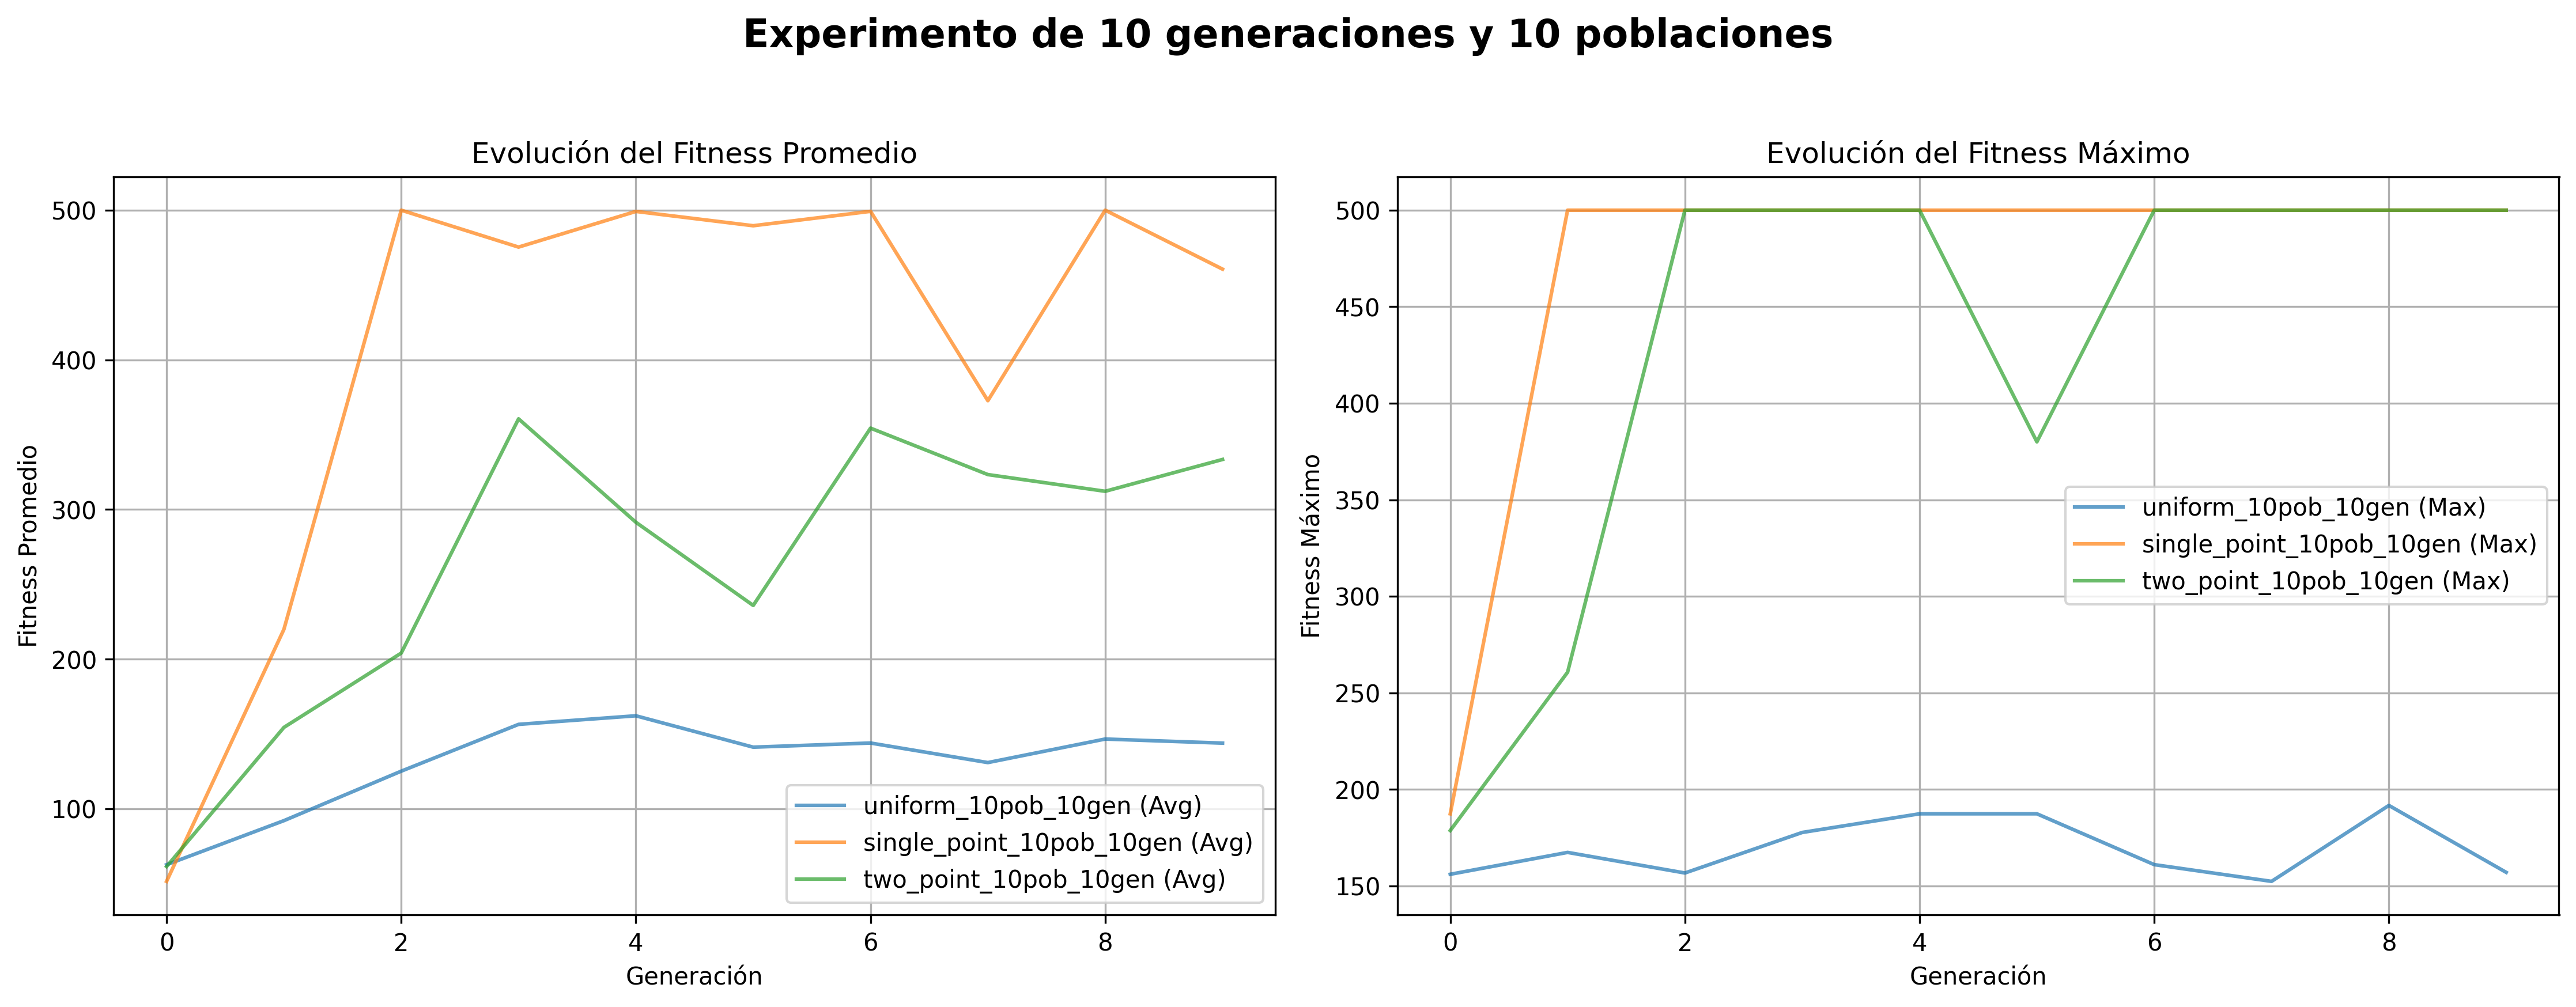
\includegraphics[width=1\textwidth]{img/10-gen-10-pob-results.png}
  \caption{Resultados de entrenamiento del CartPole con configurqcion de 10 generaciones y 10 poblaciones.}
\end{figure}

\begin{figure}[H]
  \centering
  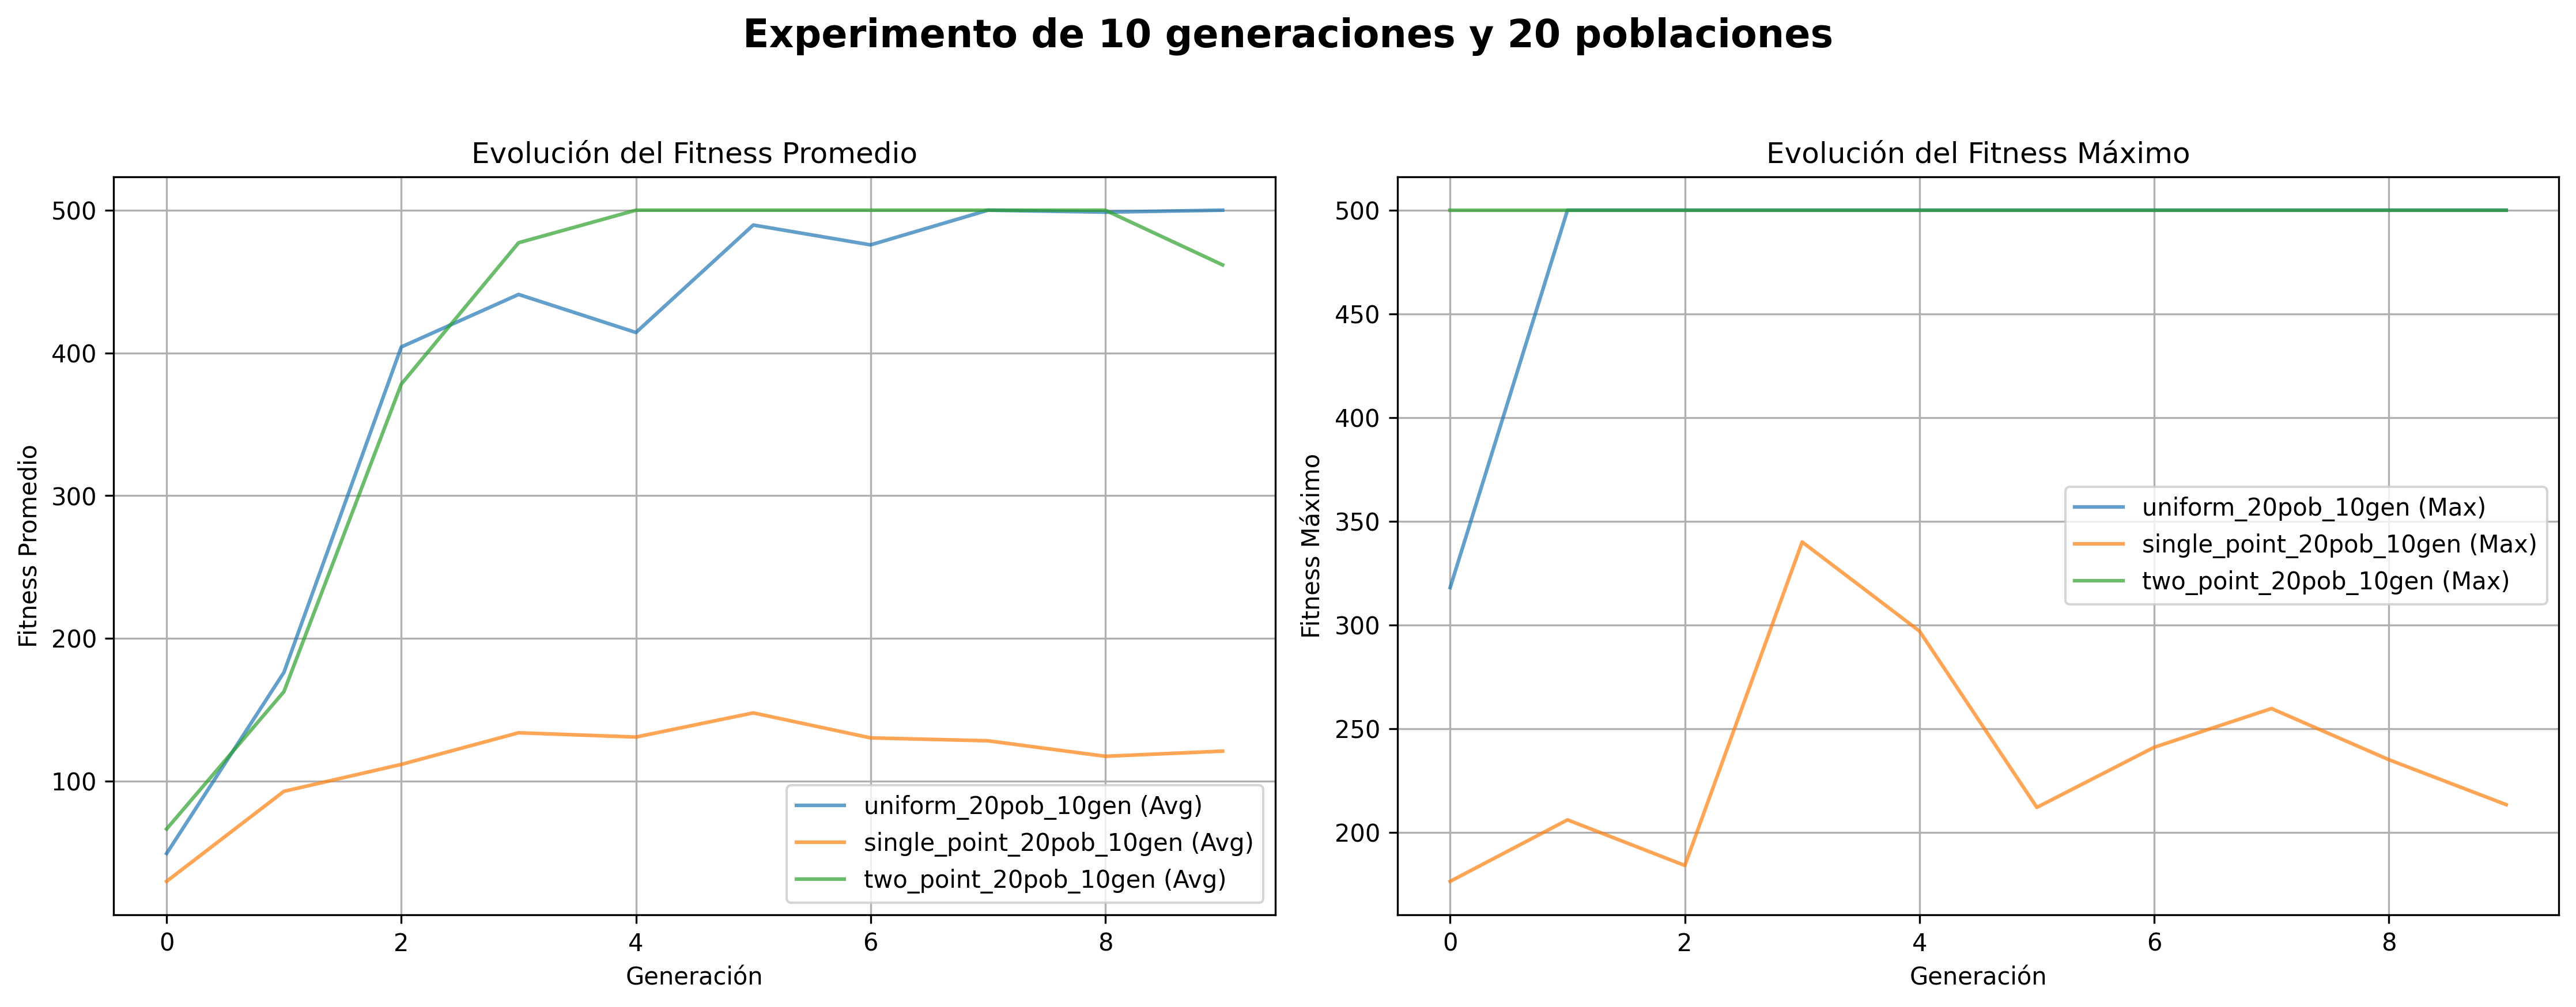
\includegraphics[width=1\textwidth]{img/10-gen-20-pob-results.png}
  \caption{Resultados de entrenamiento del CartPole con configurqcion de 10 generaciones y 20 poblaciones.}
\end{figure}

\begin{figure}[H]
  \centering
  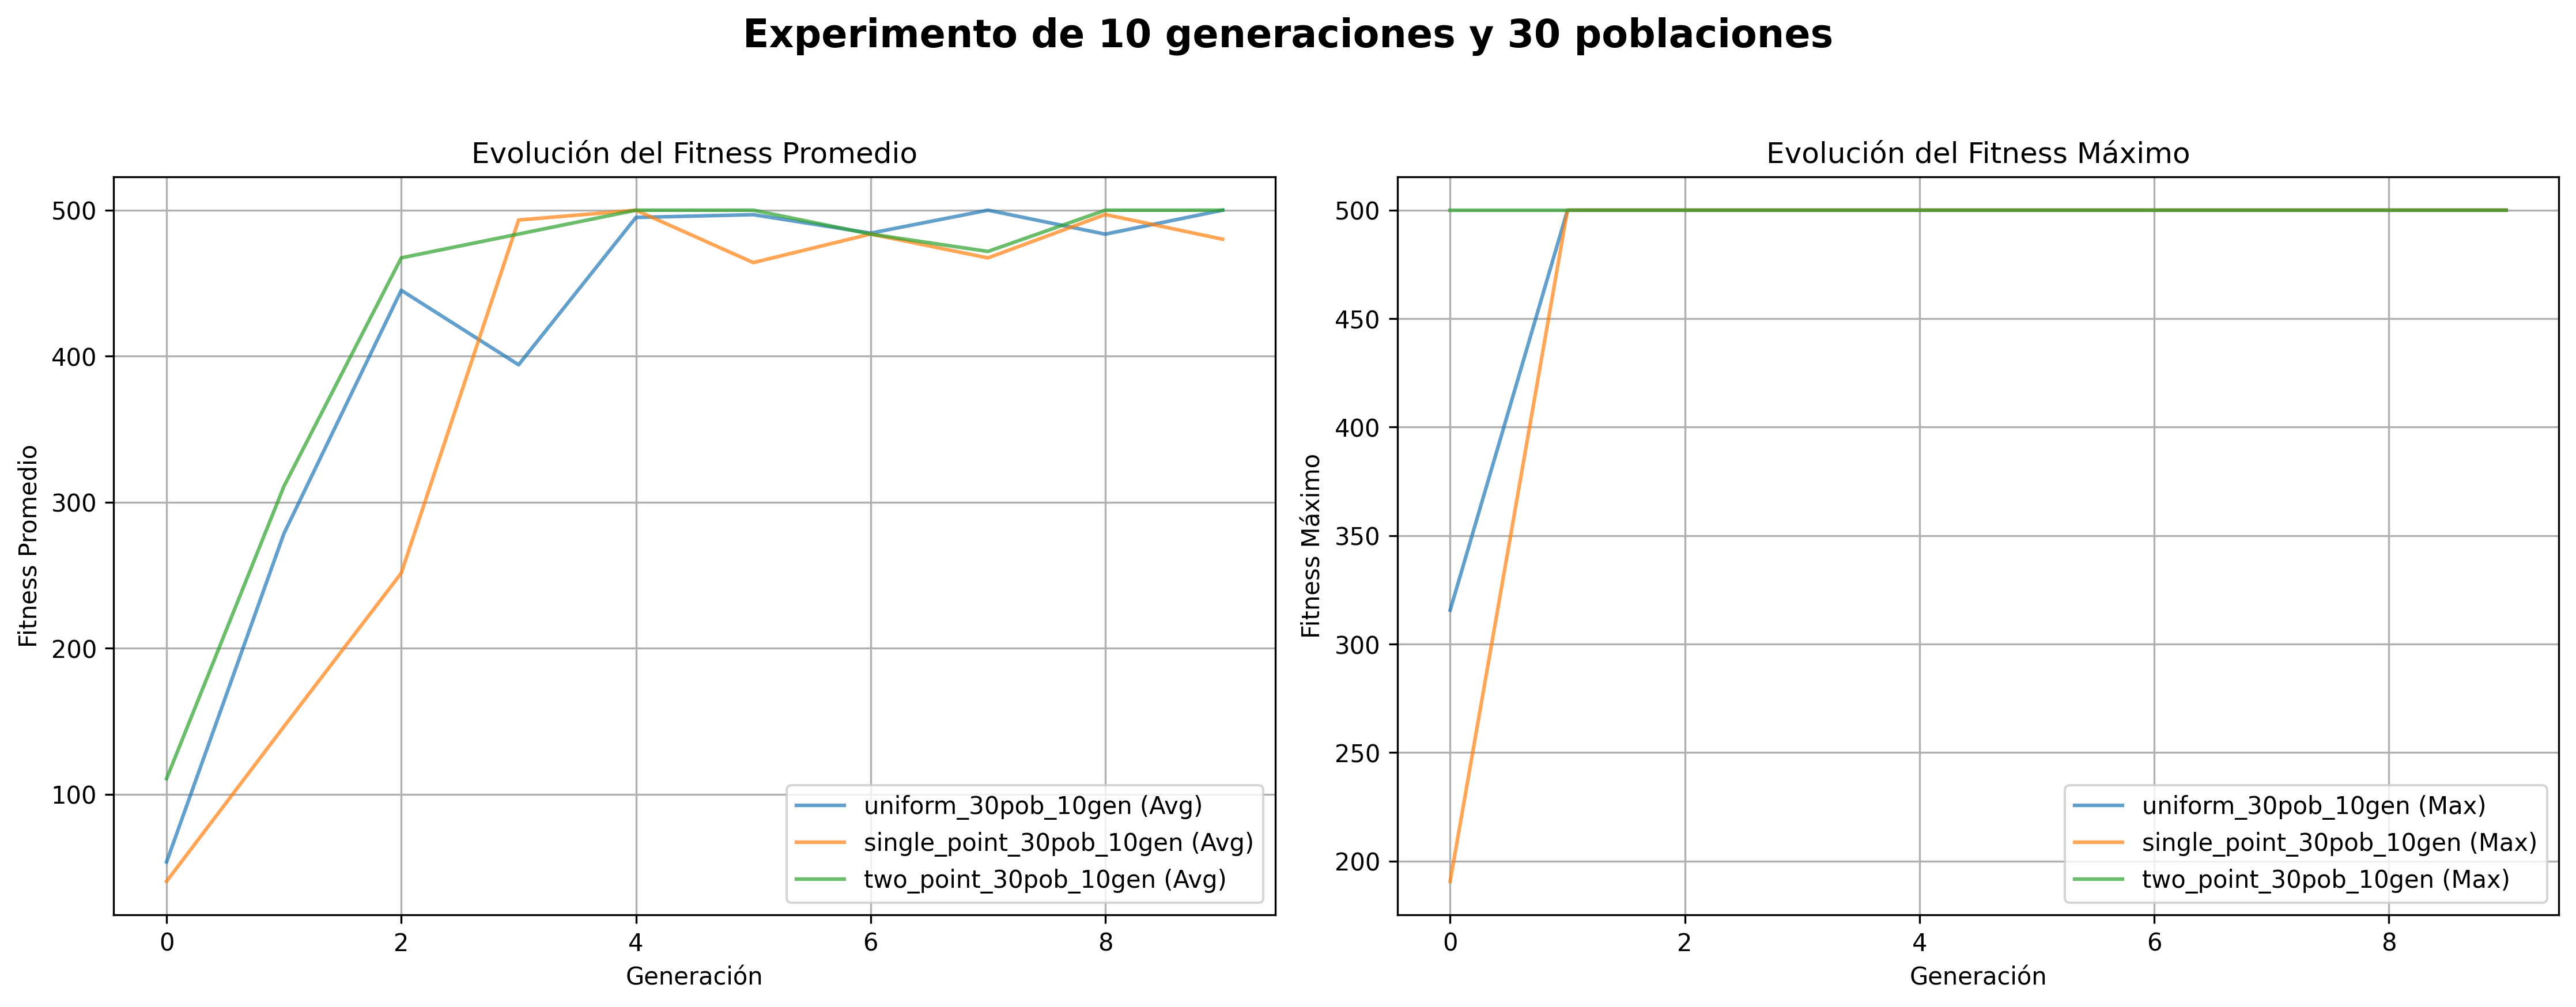
\includegraphics[width=1\textwidth]{img/10-gen-30-pob-results.png}
  \caption{Resultados de entrenamiento del CartPole con configurqcion de 10 generaciones y 30 poblaciones.}
\end{figure}

\begin{figure}[H]
  \centering
  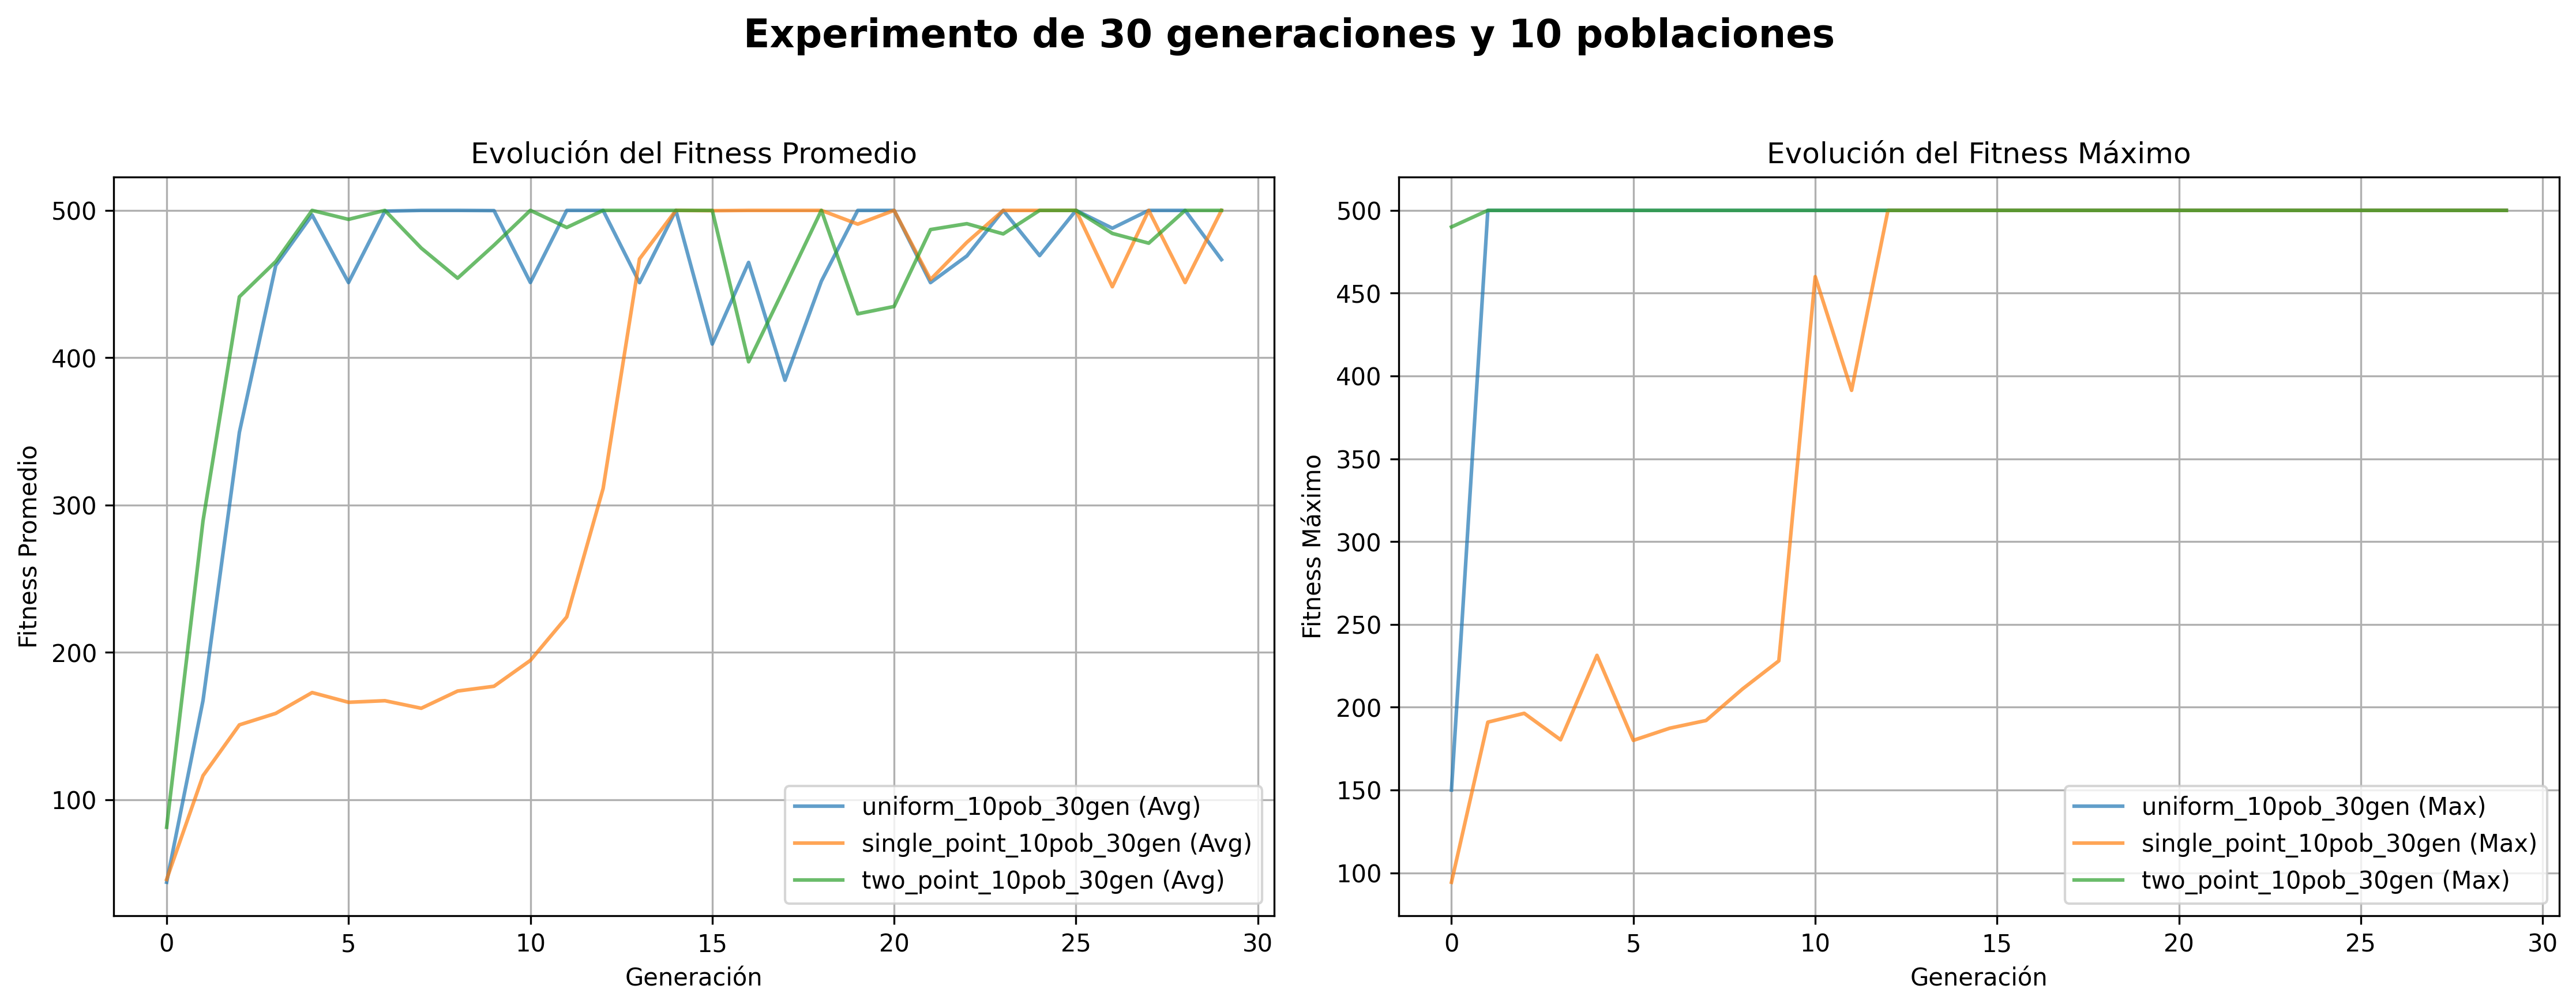
\includegraphics[width=1\textwidth]{img/30-gen-10-pob-results.png}
  \caption{Resultados de entrenamiento del CartPole con configurqcion de 30 generaciones y 10 poblaciones.}
\end{figure}

\begin{figure}[H]
  \centering
  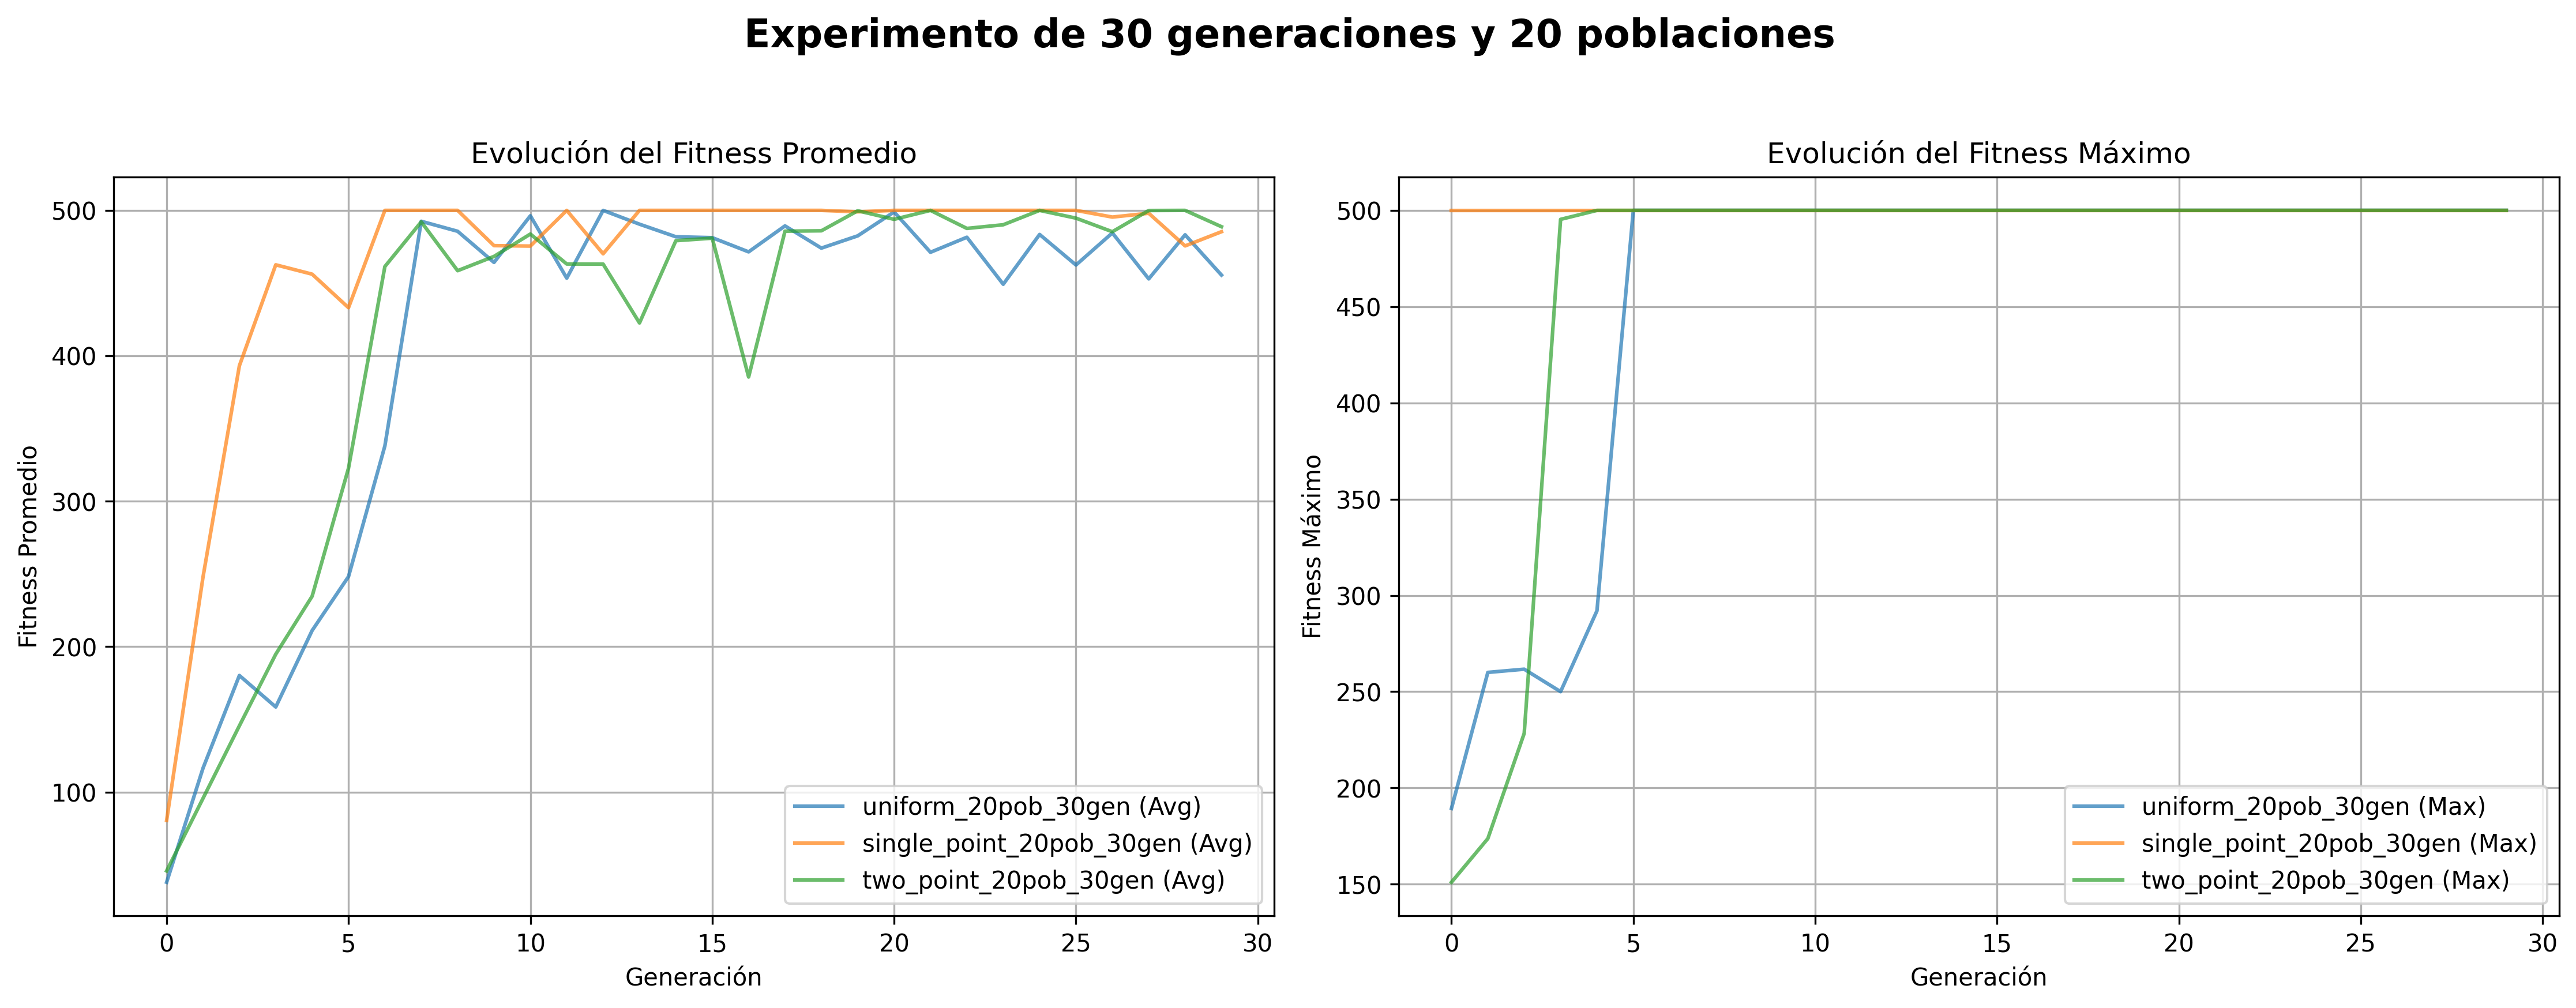
\includegraphics[width=1\textwidth]{img/30-gen-20-pob-results.png}
  \caption{Resultados de entrenamiento del CartPole con configurqcion de 30 generaciones y 20 poblaciones.}
\end{figure}

\begin{figure}[H]
  \centering
  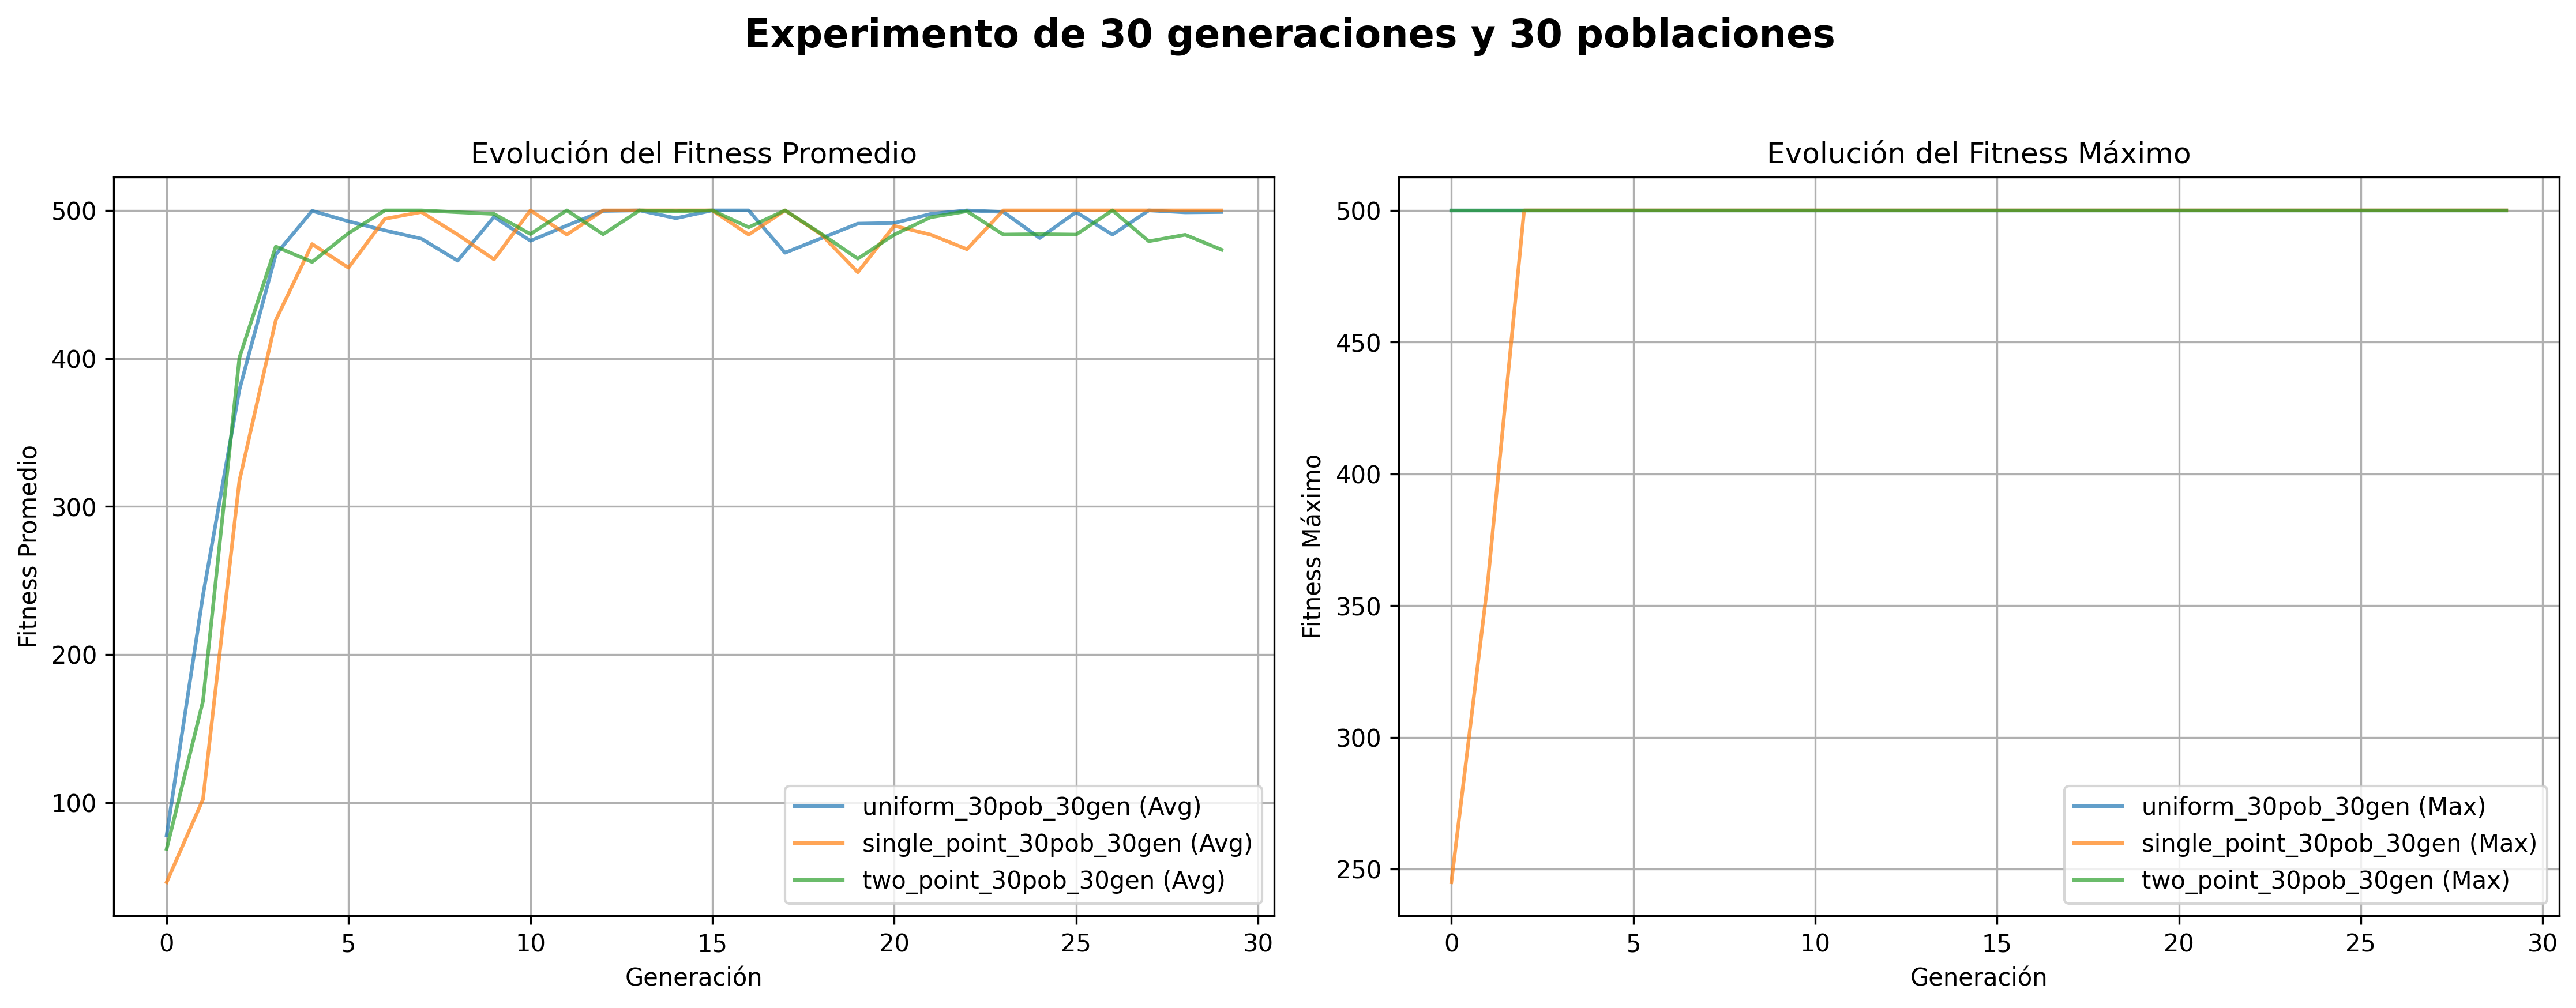
\includegraphics[width=1\textwidth]{img/30-gen-30-pob-results.png}
  \caption{Resultados de entrenamiento del CartPole con configurqcion de 30 generaciones y 30 poblaciones.}
\end{figure}

\begin{figure}[H]
  \centering
  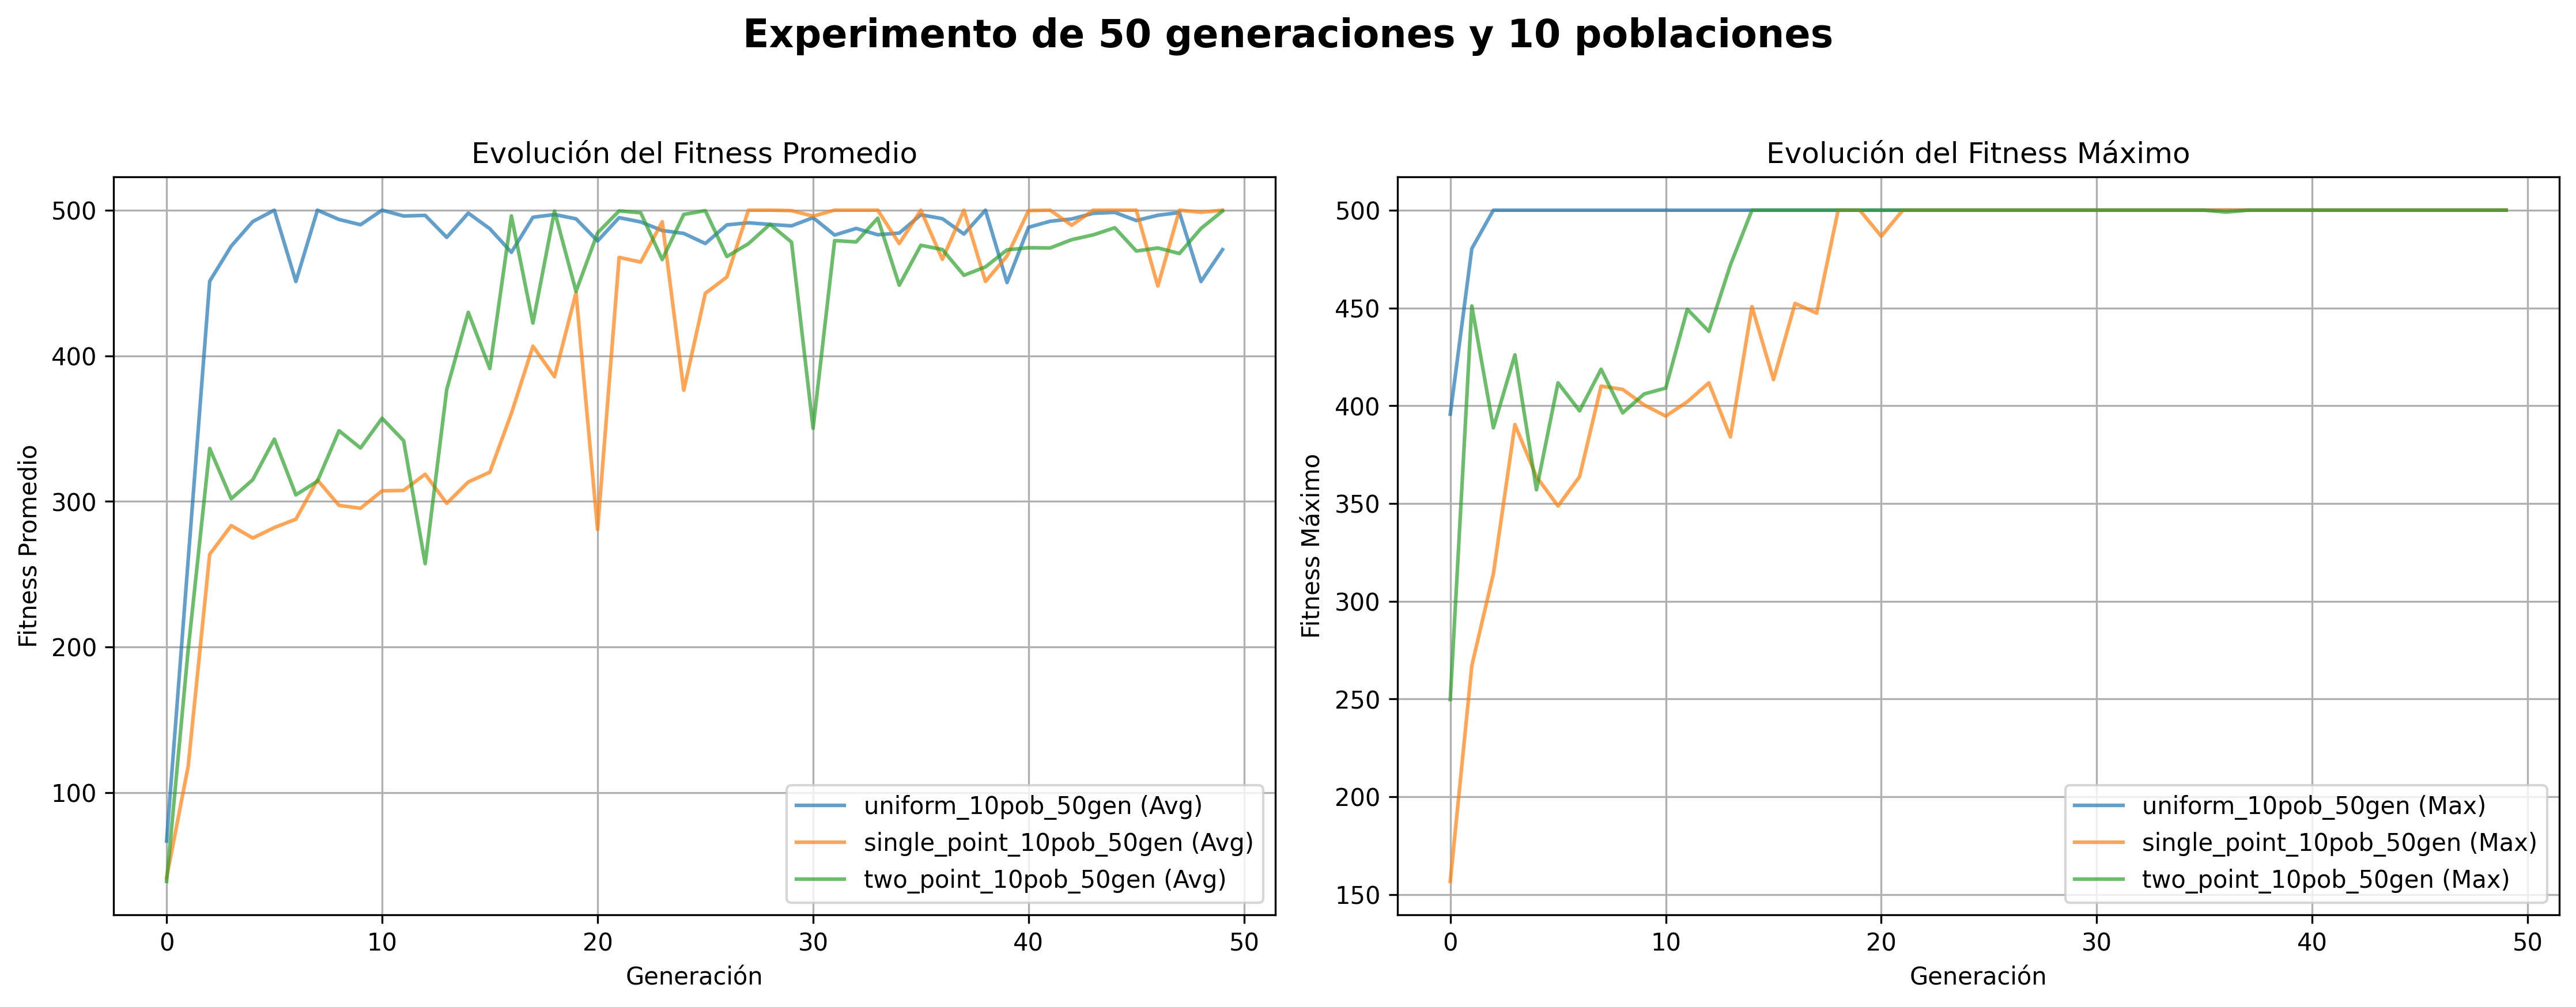
\includegraphics[width=1\textwidth]{img/50-gen-10-pob-results.png}
  \caption{Resultados de entrenamiento del CartPole con configurqcion de 50 generaciones y 10 poblaciones.}
\end{figure}

\begin{figure}[H]
  \centering
  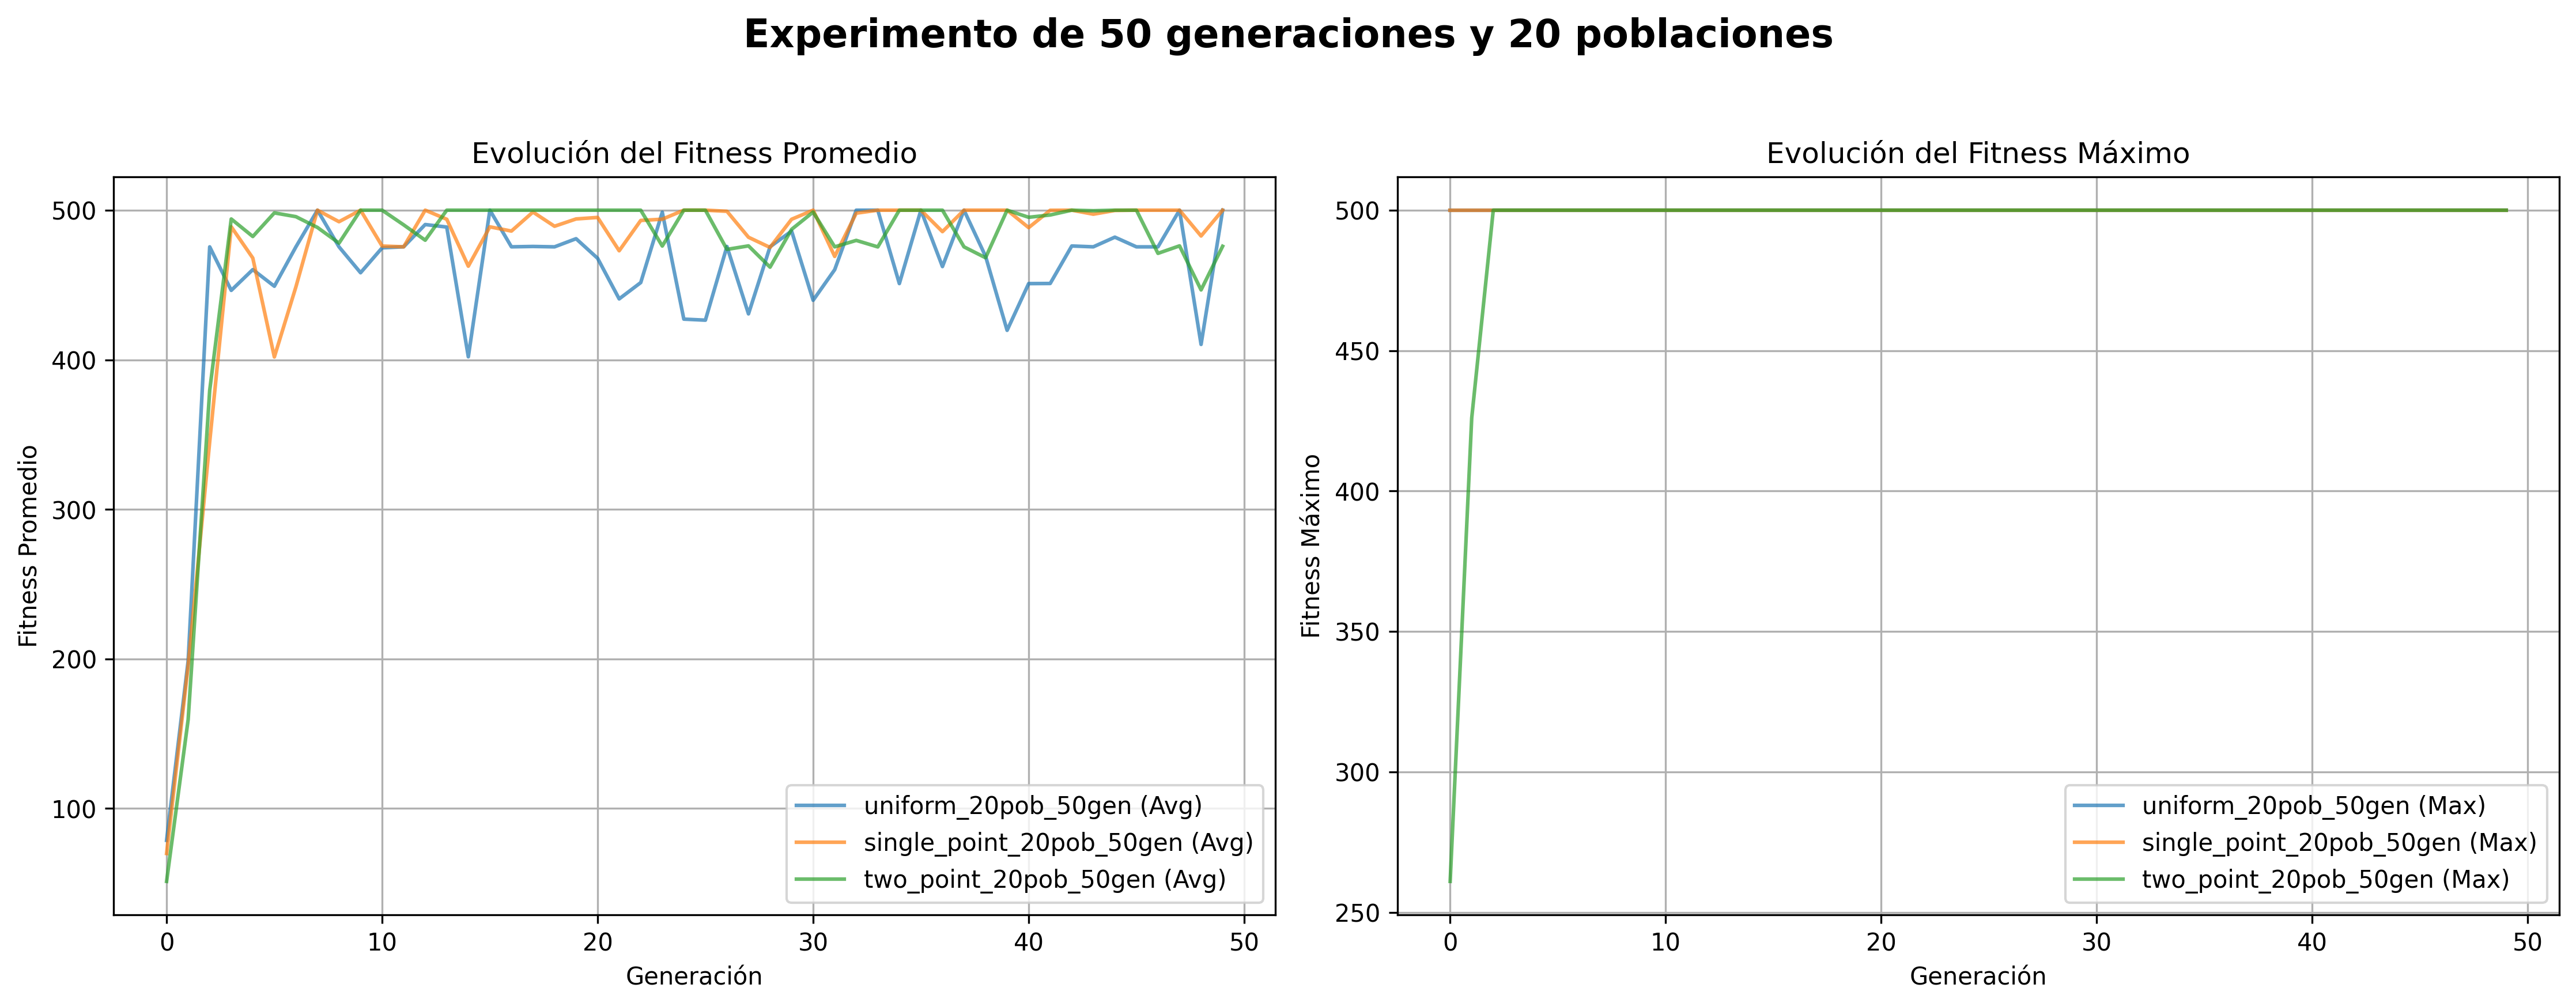
\includegraphics[width=1\textwidth]{img/50-gen-20-pob-results.png}
  \caption{Resultados de entrenamiento del CartPole con configurqcion de 50 generaciones y 20 poblaciones.}
\end{figure}

\begin{figure}[H]
  \centering
  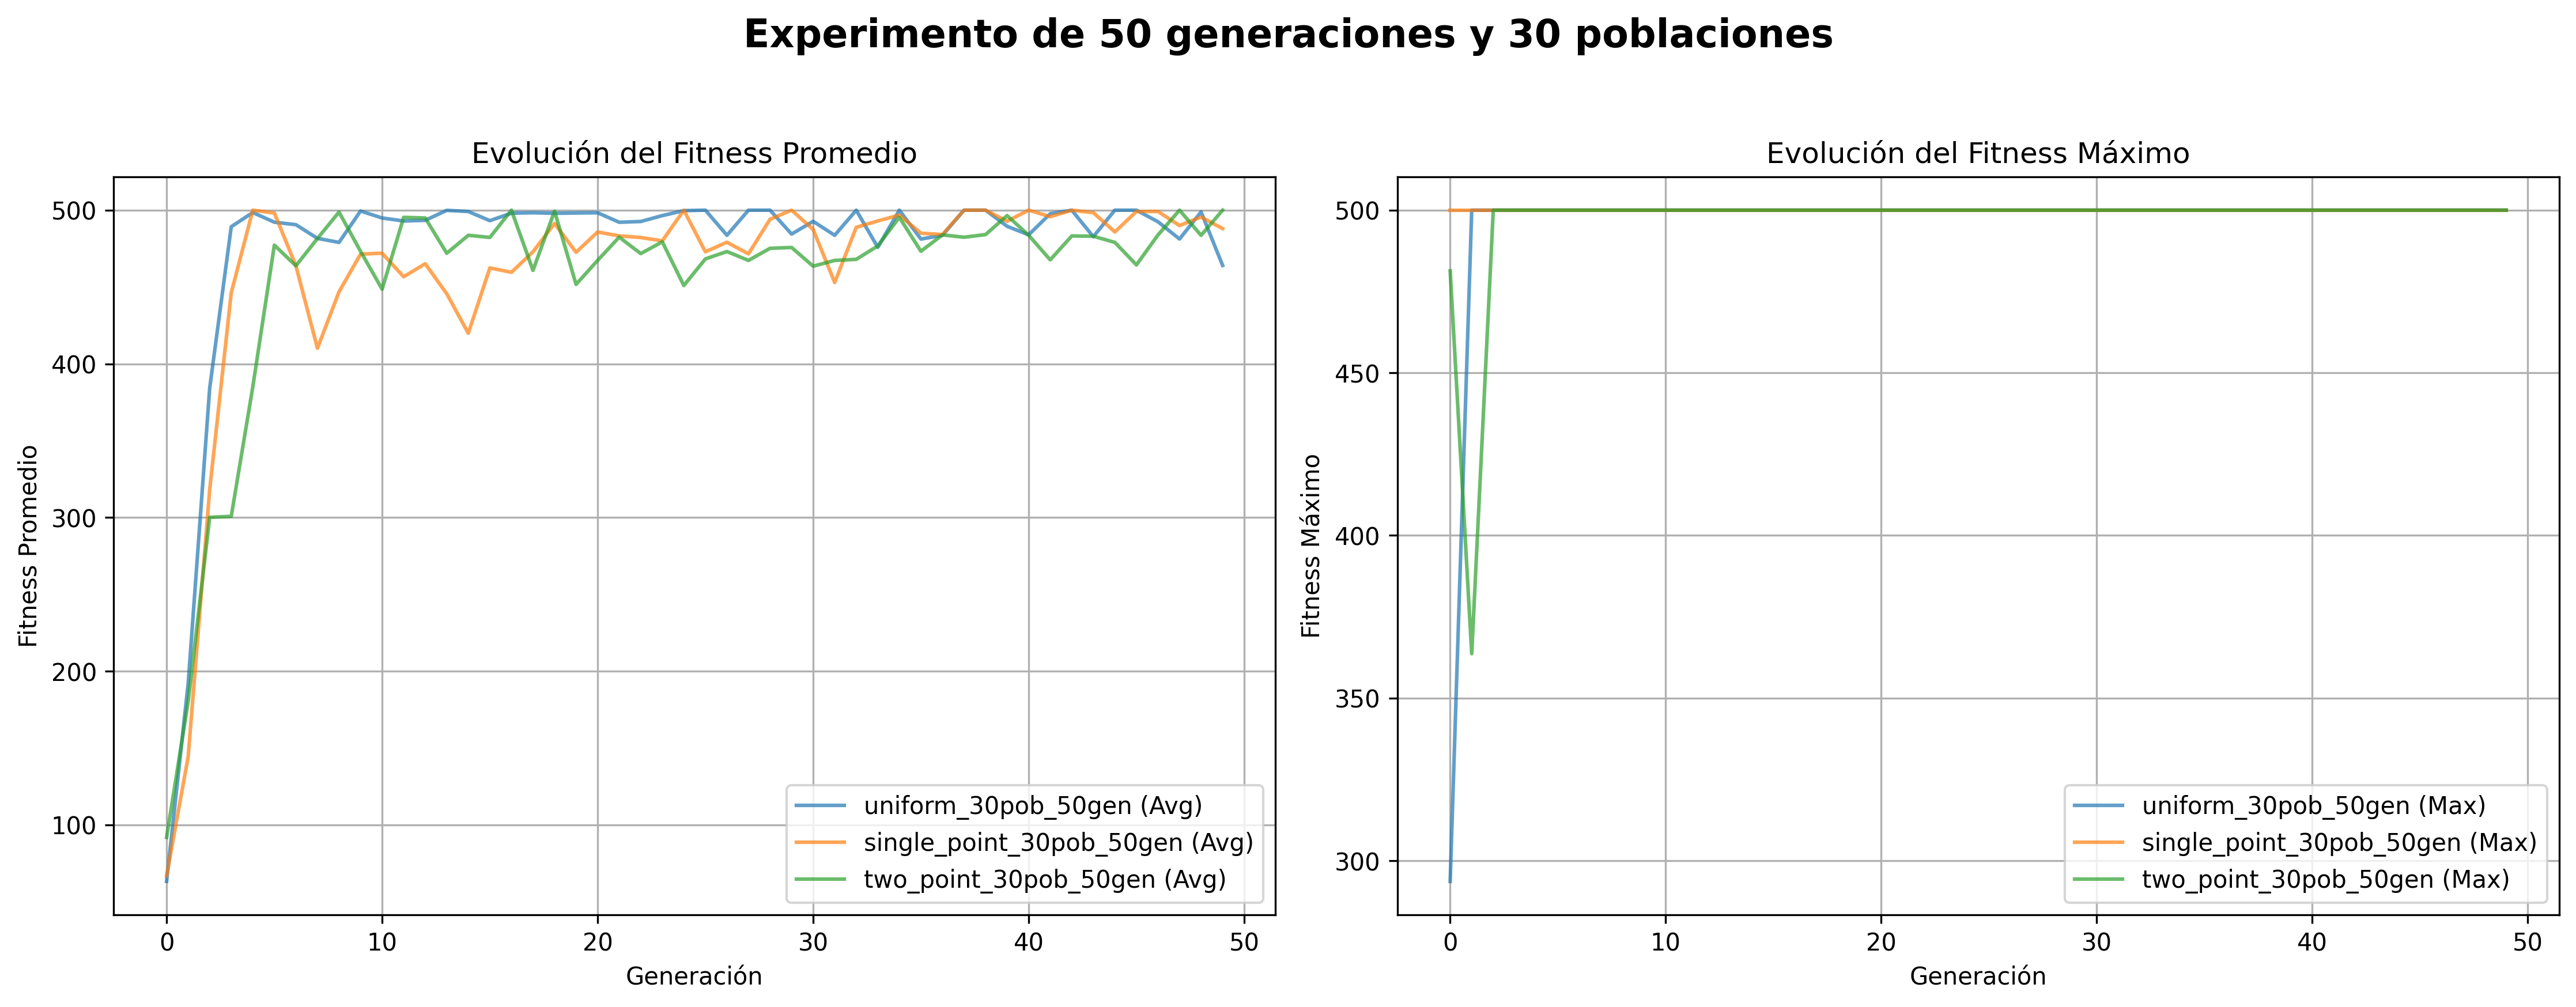
\includegraphics[width=1\textwidth]{img/50-gen-30-pob-results.png}
  \caption{Resultados de entrenamiento del CartPole con configurqcion de 50 generaciones y 30 poblaciones.}
\end{figure}

\section{Discusión crítica y análisis}
Los resultados experimentales revelan que múltiples configuraciones lograron alcanzar el fitness máximo de 500 pasos, indicando convergencia exitosa hacia políticas de control efectivas. Sin embargo, alcanzar el máximo puntaje no es el único criterio de éxito, ya que existen diferencias cualitativas en el comportamiento del agente.

El análisis crítico debe considerar varios aspectos:

\begin{itemize}
    \item \textbf{Estabilidad del control:} Aunque varios modelos alcanzaron 500 pasos, difieren en la suavidad y estabilidad de sus movimientos. Algunos agentes mantienen el poste equilibrado con movimientos mínimos y eficientes, mientras otros requieren correcciones constantes y bruscas.
    \item \textbf{Robustez:} La evaluación mediante múltiples episodios ayuda a identificar políticas consistentes versus aquellas que funcionan esporádicamente. Modelos con alta varianza entre episodios sugieren soluciones menos robustas.
    \item \textbf{Eficiencia computacional:} Las configuraciones con poblaciones más grandes (30 individuos) y más generaciones (50) requieren significativamente más tiempo de cómputo, pero no necesariamente producen mejores resultados que configuraciones más modestas.
    \item \textbf{Métodos de crossover:} Los tres métodos implementados muestran diferencias en velocidad de convergencia y exploración del espacio de soluciones. El crossover uniforme tiende a mantener mayor diversidad, mientras que los métodos de punto preservan mejor los bloques de construcción genéticos.
\end{itemize}

\section{Conclusiones y trabajo futuro}
Los algoritmos genéticos demostraron ser efectivos para resolver el problema de control de CartPole cuando se configuran apropiadamente. La simplicidad de la representación cromosómica (4 pesos) permite una evolución eficiente hacia políticas de control competentes.

\subsection*{Conclusiones principales}
\begin{itemize}
    \item Configuraciones modestas (20-30 individuos, 30-50 generaciones) son suficientes para alcanzar soluciones óptimas.
    \item La paralelización reduce significativamente los tiempos de entrenamiento, haciendo factible la experimentación exhaustiva.
    \item Los diferentes métodos de crossover ofrecen trade-offs entre exploración y explotación del espacio de búsqueda.
    \item La evaluación multi-episodio mejora la selección de políticas robustas.
\end{itemize}

\subsection*{Trabajo futuro}
\begin{itemize}
    \item Implementar representaciones cromosómicas más complejas (redes neuronales pequeñas).
    \item Evaluar algoritmos genéticos en entornos de control más desafiantes.
    \item Desarrollar métricas de calidad que consideren la eficiencia energética del control.
    \item Comparar directamente con métodos de aprendizaje por refuerzo clásicos (Q-learning, Policy Gradient).
    \item Investigar técnicas de co-evolución para balancear múltiples objetivos de control.
\end{itemize}



\end{document}

